\documentclass[12pt]{article}

\setlength{\parskip}{1em}

\usepackage[T1]{fontenc}
\usepackage[utf8]{inputenc}
\usepackage[a4paper, margin=0.7in]{geometry}
\usepackage{amsfonts}
\usepackage{mathabx}
\usepackage{listings}
\usepackage{xcolor}
\usepackage{subcaption}
\usepackage{multirow}
\usepackage{makecell}
\usepackage{float}
\usepackage{graphicx}

\usepackage{hyperref}
\hypersetup{
  colorlinks=true,
  linkcolor=blue,
  urlcolor=blue,
  pdftitle={PC40 Hands-on: UPC}
}

% \definecolor{gray}{rgb}{0.5,0.5,0.5}
% \definecolor{purple}{rgb}{0.58,0,0.82}
\definecolor{bgColor}{rgb}{0.95,0.95,0.92}
\lstdefinestyle{C}{
    backgroundcolor=\color{bgColor},
    commentstyle=\color{gray},
    keywordstyle=\color{magenta},
    numberstyle=\tiny\color{gray},
    stringstyle=\color{purple},
    basicstyle=\footnotesize,
    breakatwhitespace=false,
    breaklines=true,
    captionpos=b,
    keepspaces=true,
    numbers=left,
    numbersep=5pt,
    showspaces=false,
    showstringspaces=false,
    showtabs=false,
    tabsize=2,
    language=C
}

\newcommand{\us}[0]{${\mu}s$}

\title{SY40: Rapport de projet}
\author{Adrien Burgun}
\date{Automne 2021}

\graphicspath{{report/}}

\begin{document}
\maketitle

\begin{abstract}
    Pour ce projet, nous avons dû modéliser et implémenter une plateforme multi-modale, avec pour particularité la présence de deux grues, qui doivent opérer en parallèle.

    Nous verrons en premier temps la modélisation, puis en deuxième temps l'implémentation et les résultats de celle-ci.
    Enfin, nous concluerons avec mon retour d'expérience.

    Le code source du projet ainsi que de ce rapport peuvent être trouvés sur la repository de ce projet:
    \url{https://github.com/adri326/sy40-project}
\end{abstract}

\newpage
\tableofcontents
\newpage

\section{Modélisation}
\label{sec:modelisation}

Le projet avait les contraintes suivantes:

\begin{itemize}
    \item Deux grues doivent opérer sur une plateforme multimodale
    \item Il y a une voie bidirectionelle de bateau, avec un maximum de $2$ bateaux stationnés
    \item Il y a une voie unidirectionelle de trains, avec un maximum de $2$ trains présents sur le quai
    \item Il y a une voie de voitures, avec un maximum de $M$ voitures
    \item Les containers doivent être déchargés de leur mode de transport puis chargé sur un autre mode de transport s'il y a de la place
    \item L'orientation des véhicules importe
    \item Les trains ont au plus $N$ wagons
    \item La concurrence doit être gérée proprement
    \item Les grues ne peuvent pas se croiser ou se téléscoper
\end{itemize}

À partir de ces règles, j'ai décidé de prendre certaines libertés (dont quelques unes qui seraient dubieuses à mettre en place dans la vie réelle):

\begin{itemize}
    \item La plateforme est séparée en deux parties, et chaque grue est confinée dans l'une des deux parties.
    \item Une tour de contrôle est ajoutée, qui va appeler de nouveaux véhicules et faire partir les véhicules pleins. La tour de contrôle ignore la courbature de la Terre. La tour de contrôle peut communiquer avec les deux grues, qu'importe leur position.
    \item La voie maritime est supposée infinie, et une infinité de bateaux peuvent attendre dans le canal, voile fermée et ancre baissée, jusqu'à ce qu'il y ait de la place, dans quel cas tous les bateaux avancent d'unisson d'une case. Les navigateurs ne dorment jamais.
    \item La voie routière est transformée en un parking (théoriquement infini) ainsi qu'une zone de chargement/déchargement. Les routiers reçoivent un beepeur et le beepeur appairé se passe entre les deux grues et la tour de contrôle. Les routiers ne dorment jamais.
    \item Les containers stockent leurs destination dans un nombre; les bateaux, camions, trains et wagons stockent également leur propre destination.
    \item Les grues sont spécialisées: l'une charge le train et décharge les bateaux, tandis que l'autre charge les bateaux et décharge le train.
    \item Les bateaux peuvent être ammenés à revenir derrière la file, ce qui permet d'améliorer grandement la qualité des solutions.
    \item Les conducteurs de trains et les opérateurs de grue ne dorment jamais (ils peuvent aussi se relayer, mais instantanément).
    \item Les opérateurs de la tour de contrôle peuvent dormir.
\end{itemize}


\subsection{Organisation}

Les deux grues reçoivent un nom: Alpha ($\alpha$) et Beta ($\beta$).
La tour de contrôle est quand à elle nommée Gamma ($\gamma$).

\begin{figure}[H]
    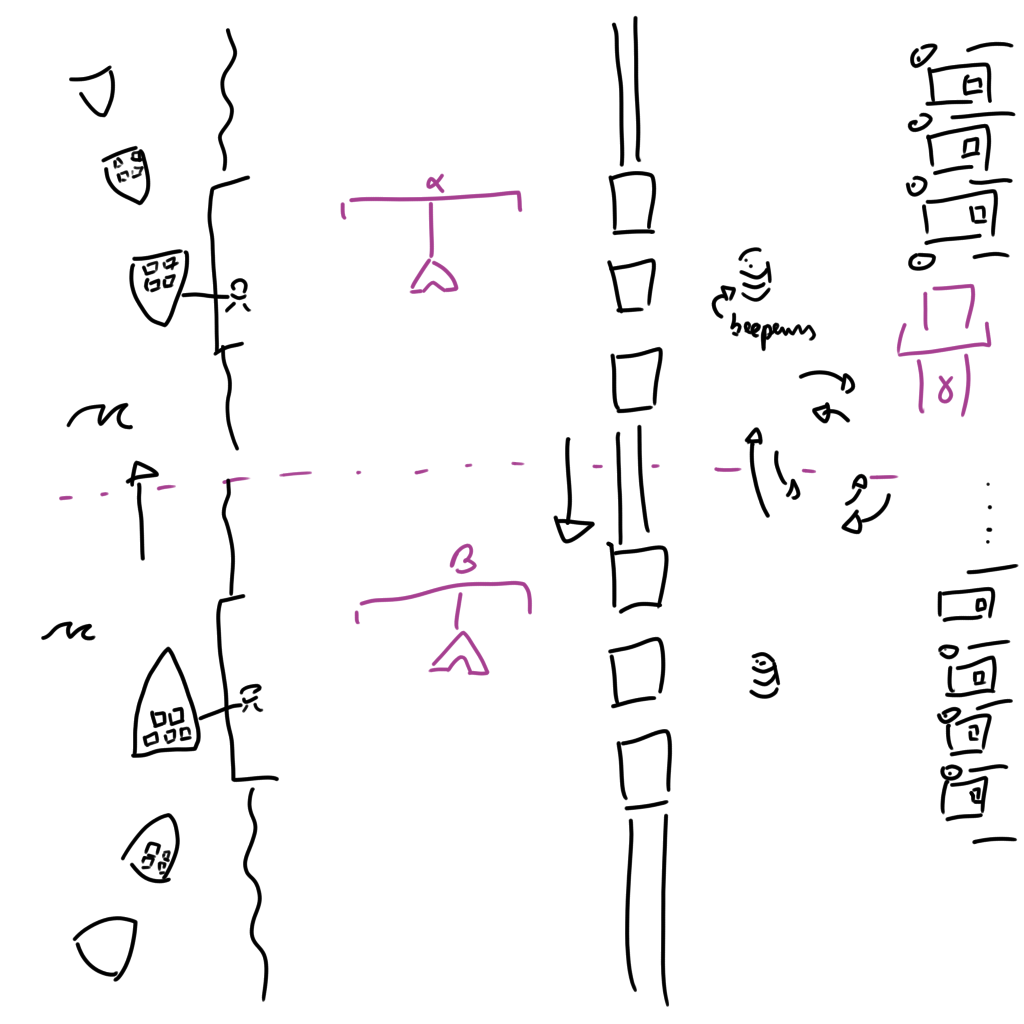
\includegraphics[width=0.95\columnwidth]{schema.png}
    \caption{Schéma global\label{fig:schema}}
\end{figure}

\subsection{Trains}

La voie de train consiste en deux listes contigues de \texttt{wagons}, pouvant accueillir si besoin l'entièreté de deux trains.
$\gamma$ stocke de son côté la liste entière des wagons et des informations sur ceux-cis (s'ils ont été vidés, remplis, etc.)

$\beta$ décharge les wagons; lorsqu'un wagon est vide, un message (\textsc{wagon\_empty}) est envoyé à $\gamma$.

Si $\gamma$ voit que des wagons peuvent être avancés, il bloque le mutex de la voie de trains de $\beta$ et de $\alpha$, et il fait avancer les wagons pour que $\alpha$ puisse commencer à les remplir.

$\alpha$ charge les wagons; lorsqu'un wagon est vide, un message (\textsc{wagon\_full}) est envoyé à $\gamma$.

Si $\gamma$ voit que tous les wagons d'un train est rempli, il bloque le mutex de $\alpha$ et fait partir le train, avant de bloquer le mutex de $\beta$ pour lui donner un nouveau train.

\subsection{Bateaux}

Les bateaux sont similaires aux trains, à la différence que la restriction sur les wagons est enlevée.
Deux \texttt{VecDeque} (double-ended queues) sont crées, une pour $\alpha$ et une pour $\beta$. $\alpha$ et $\beta$ possèdent également un bateau ammaré, stocké séparément.
Chaque \texttt{VecDeque} est placé derrière un mutex (dans le réseau plus bas, labellés $S(\alpha)$ et $S(\beta)$).

$\alpha$ décharge les bateaux (et charge les wagons) un à un; lorsqu'un bateau est vidé, le bateau est désamarré et la tour de contrôle indique au bateau de se mettre en file chez $\beta$.

$\beta$ charge les bateaux (et décharge les wagons) un à un; lorsqu'un bateau est rempli, le bateau est désamarré et la tour de contrôle indique au bateau qu'il peut partir.

Voici le réseau de Petri correspondant à l'opération de déchargement d'un bateau:

\begin{figure}[H]
    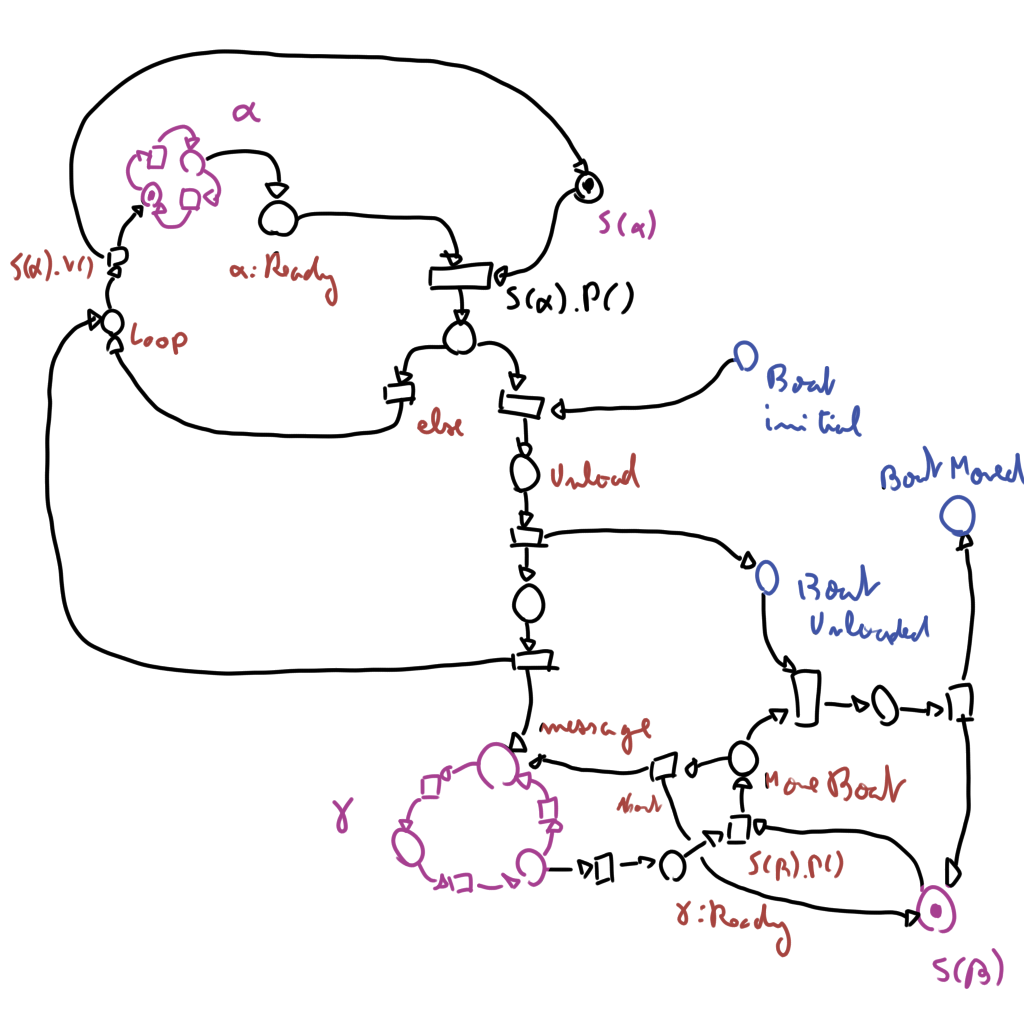
\includegraphics[width=0.95\columnwidth]{boat.png}
    \caption{Réseau de Petri pour l'opération de déchargement d'un bateau\label{fig:petri-boat}}
\end{figure}

\subsection{Camions}

Les camions sont tous stockés dans une seule liste contigue.
Des pointeurs vers ces camions sont distribués à $\alpha$, $\beta$ et $\gamma$: on garantit alors qu'il n'existe qu'un pointeur (en dehors de la liste mère) vers chaque camion.

$\alpha$ et $\beta$ déchargent et chargent les camions, en fonction de leur état. Lorsqu'un camion est vidé, il est envoyé à $\gamma$, qui l'envoie à l'autre grue.
Lorsqu'un camion est rempli, il est envoyé à $\gamma$, qui crée un nouveau camion.

Les camions sont transmis via des messages; il est possible de représenter une opération de déchargement + chargement d'un camion avec le réseau de Petri suivant:

\begin{figure}[H]
    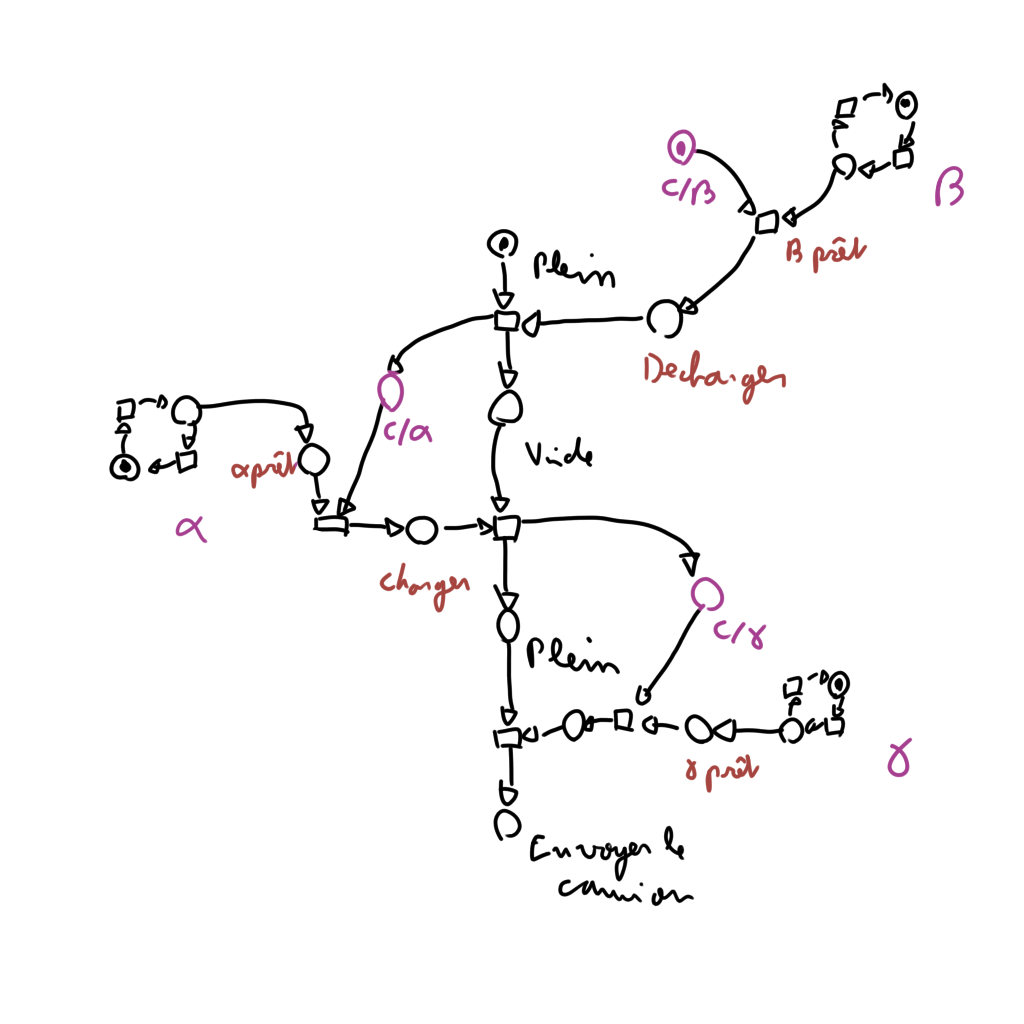
\includegraphics[width=0.95\columnwidth]{truck.png}
    \caption{Réseau de Petri pour l'opération de déchargement et chargement d'un camion. $C/\alpha$, $C/\beta$ et $C/\gamma$ représentent la possession du pointeur vers le camion\label{fig:petri-truck}}
\end{figure}

\subsection{Messages}

$\alpha$ et $\beta$ peuvent tous les deux envoyer des messages à $\gamma$ (1), et $\gamma$ peut répondre (2).

$\gamma$ dort la pluspart du temps; il est reveillé via un moniteur.
On définit une file de message $Q(\gamma)$ (implémentée à la main avec une liste chaînée), un mutex $S(\gamma)$ et un moniteur $M(\gamma)$:

\begin{figure}[H]
    \begin{lstlisting}[language=C, literate={γ}{$\gamma$}1 {α}{$\alpha$}1 {β}{$\beta$}1 {à}{{\`a}}1 {é}{{\'e}}1]
    Fucntion send_γ(message):
        S(γ).P() // Risque de deadlock: il est important que
        // ni S(α) ni S(β) ne soient bloqués à ce moment par le thread
        Q(γ).push(message)
        M(γ).signal()

    Boucle dans γ:
        S(γ).P()
        M(γ).wait(S(γ))
        message = Q(γ).pop()
        S(γ).V()
        // Gérer le message
    \end{lstlisting}
\end{figure}

$\alpha$ et $\beta$ ne dorment jamais, donc la communication vers eux est plus simple. $\alpha$ et $\beta$ ont chacun un mutex ($S(\alpha)$ et $S(\beta)$) et une file de message ($Q(\alpha)$ et $Q(\beta)$):

\begin{figure}[H]
    \begin{lstlisting}[language=C, literate={γ}{$\gamma$}1 {α}{$\alpha$}1 {β}{$\beta$}1 {τ}{$\tau$}1 {à}{{\`a}}1 {é}{{\'e}}1]
    Function send(message, τ: α|β):
        S(τ).P() // Risque de deadlock: il est important que S(γ)
        // ne soit pas bloqué à ce moment
        Q(τ).send(message)
        S(τ).V()

    Boucle dans τ:
        S(τ).P()
        message = Q(τ).read()
        S(τ).V()
        // Gérer le message
    \end{lstlisting}
\end{figure}

\subsection{Simulation des réseaux}

En parallèle de ce projet, j'ai écrit une librairie pour simuler les réseaux de Petri de manière automatique.
La librairie permet de résoudre les conflits et elle arrive à générer le graphe de tous les états du réseau.

Les réseaux sont entrés sous forme de code, ce qui permet de les paramétriser.
Les boucles visibles sur les réseaux peuvent notamment varier de longueur.

Il est alors possible de vérifier que des invariantes sont respectées par chaque réseau, et ce pour différentes valeurs de paramètres. Par exemple:

\begin{itemize}
    \item Les mutex ne sont pas libérés plus d'une fois
    \item Seul un jeton se trouve dans une section critique à la fois
    \item Un état final avec succès est toujours atteint (le véhicule est déchargé et tous les mutex sont libérés)
\end{itemize}

Les tests ont été automatisés et peuvent être lancés avec l'outil \texttt{cargo test --release}.
Quatre réseaux sont testés de cette manière: deux pour chaqu'un des réseaux présentés dans ce document, contenant pour l'un la partie déchargement, et pour l'autre la partie déchargement + chargement.

Il est possible de faire afficher le graphe de tous les états atteints par l'automate simulant le Réseau de Petri:

\begin{figure}[H]
    \centering
    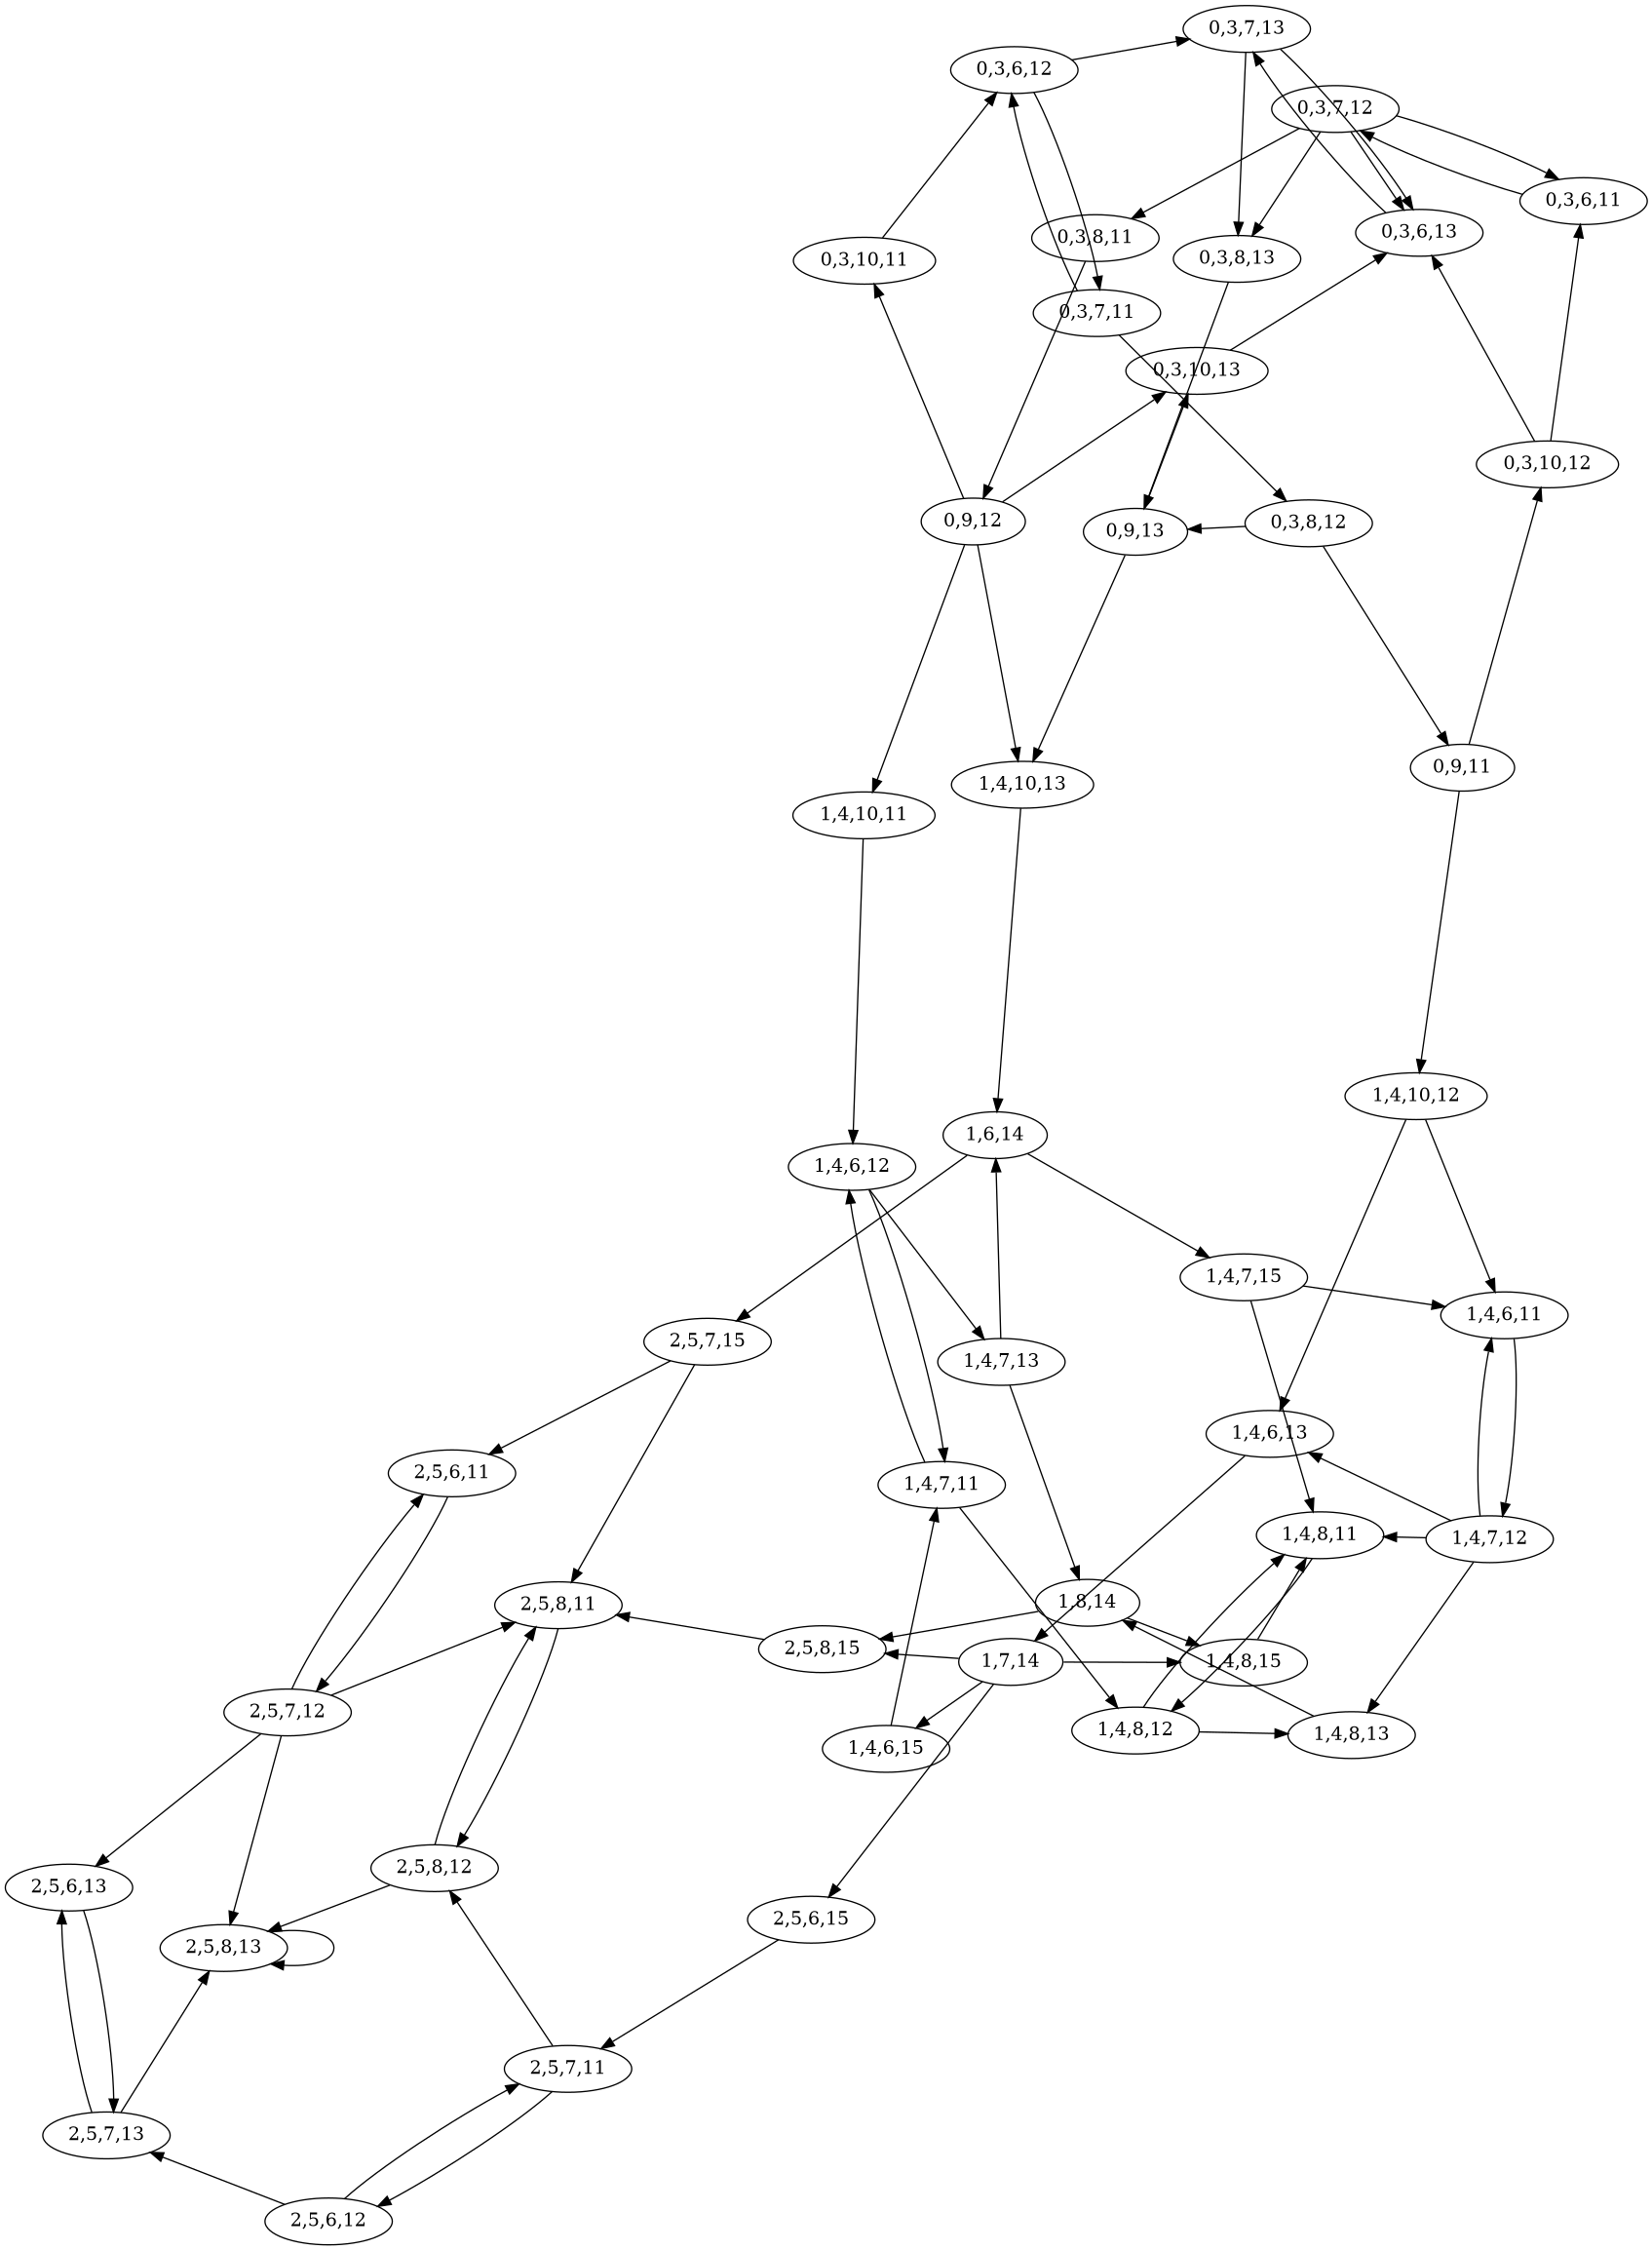
\includegraphics[width=0.5\columnwidth]{petri-graph.png}
    \caption{Le graphe de tous les états atteints par le réseau de Petri pour les camions. La taille des graphes explose lorsque le réseau grandit, celui-ci est un des plus petits. Les propriétés sont heureusement vérifiées automatiquement, mais on peut voir que tous les états convergent vers l'état "2, 5, 8, 13".\label{fig:petri-graph}}
\end{figure}

\section{Implémentation}

Le projet a été séparé en un ensemble de fichiers, chacun gérant une partie du projet.
Un style de code lisible a été maintenu.

Une librairie, \texttt{ulid} (Universally Unique Lexicographically Sortable Identifier), a été utilisée pour donner un identifiant unique aux containers et aux véhicules.

\begin{itemize}
    \item \texttt{assert.h} contient des fonctions utilisées pour vérifier
    \item \texttt{boat.c} contient les fonctions pour les structures \texttt{boat\_t}, \texttt{boat\_lane\_t} et \texttt{boat\_deque\_t}.
    \item \texttt{container.c} gère les containers et les emplacements de containers
    \item \texttt{control\_tower.c} contient le code pour la tour de contrôle, ainsi que le code pour communiquer avec celle-ci
    \item \texttt{crane.c} contient le code pour les deux grues, ainsi que le code pour communiquer avec elles
    \item \texttt{main.c} contient le code d'initialisation du projet
    \item \texttt{message.c} contient la structure \texttt{message\_t}, utile pour communiquer entre les threads
    \item \texttt{train.c} contient les fonctions pour les structures \texttt{wagon\_t}, \texttt{train\_lane\_t} et \texttt{train\_t}.
    \item \texttt{truck.c} contient les fonctions pour les structures \texttt{truck\_t}, \texttt{truck\_ll} et \texttt{truck\_lane\_t}.
    \item \texttt{ulid.c} gère un générateur unique à chaque thread, nécessaire pour utiliser la librairie ulid.
\end{itemize}

Différends paramètres, tel que le nombre de cargo sur un bateau, ont été placés dans les fichiers \texttt{.h}, afin de facilement les modifier.

\subsection{Jeux d'essais}

Par défaut, il y a:

\begin{itemize}
    \item 5 containers par bateau
    \item 4 wagons par train
    \item 2 containers par wagon
    \item 20 bateaux
    \item 10 camions
\end{itemize}

Avec uniquement 20 bateaux et 10 camions, il est difficile pour que des véhicules soient envoyés.
Néanmoins, environ 6 véhicules sont envoyés en moyenne. Par exemple:

\begin{lstlisting}
    Truck => Bordeaux (2)
    Truck => Paris (0)
    Truck => Paris (0)
    Truck => Suez (1)
    Truck => New York (3)
    Truck => Paris (0)
\end{lstlisting}

Si l'on augment le nombre de véhicules pour avoir 50 bateaux et 50 camions, on obtient plus de résultats, avec en moyenne 53 véhicules envoyés. Par exemple:

\begin{lstlisting}
    Truck => New York (3)
    Truck => Bordeaux (2)
    Truck => Paris (0)
    Truck => Paris (0)
    ... 50 autres camions ...
    Boat => Suez (1)
    Truck => Bordeaux (2)
    Truck => Bordeaux (2)
    Truck => Paris (0)
    Truck => Paris (0)
    Truck => Singapour (4)
    ... 20 autres camions ...
    Truck => Suez (1)
\end{lstlisting}

Si l'on augmente ensuite le nombre de containers sur chaque bateau à 10, la moyenne passe cette fois-ci à 61:

\begin{lstlisting}
    Truck => New York (3)
    Truck => Bordeaux (2)
    ... 50 autres camions ...
    Train => Singapour (4)
    Truck => New York (3)
    Truck => New York (3)
    ... 15 autres camions ...
\end{lstlisting}

Si, au contraire, on donne à chaque train 10 wagons, la moyenne passe à 68.

Enfin, voici ce à quoi ressemble l'environnement d'une grue au démarrage de la simulation. Un "x" correspond à un cargo qui doit être déchargé et un "-" à un espace libre.

\begin{lstlisting}
=== Crane { load_boats = false, load_trains = true } ===
BoatLane { queue = BoatDeque { length = 21, boats = [
    (xxxxx) -> Suez (1),
    (xxxx-) -> New York (3),
    (xxxx-) -> New York (3),
    (xv---) -> Suez (1),
    (xx---) -> Suez (1),
    (xxx--) -> Singapour (4),
    (xxxx-) -> New York (3),
    (x----) -> Suez (1),
    (xx---) -> New York (3),
    (x----) -> Suez (1),
    (x----) -> Bordeaux (2),
    (xx---) -> Bordeaux (2),
    (xxx--) -> New York (3),
    (xxxx-) -> New York (3),
    (x----) -> New York (3),
    (v----) -> Paris (0),
    (xxxx-) -> Paris (0),
    (xxx--) -> Bordeaux (2),
    (x----) -> Suez (1),
    (x----) -> Suez (1),
    (xx---) -> Singapour (4)
] }, current_boat = None }
TrainLane { n_wagons = 0, wagons = [] }
TruckLane [
    <<(x) -> Suez (1),
    >>(-) -> Suez (1),
    >>(-) -> New York (3),
    <<(x) -> Suez (1),
    >>(-) -> Bordeaux (2),
]
=== ~ ===
\end{lstlisting}

Et voici ce à quoi ressemble un environnement de grue à la fin. Un "v" correspond à un container au bon endroit:

\begin{lstlisting}
=== Crane { load_boats = true, load_trains = false } ===
BoatLane { queue = BoatDeque { length = 1, boats = [
    (vv---) -> Singapour (4)
] }, current_boat = None }
TrainLane { n_wagons = 3, wagons = [
    (--) -> Singapour (4),
    (x-) -> Singapour (4),
    (--) -> Singapour (4),
] }
TruckLane [
    >>(-) -> Bordeaux (2),
    >>(-) -> Paris (0),
    >>(-) -> Paris (0),
]
=== ~ ===
\end{lstlisting}

\section{Conclusion}

J'ai été très satisfait du sujet du projet et de la modélisation que j'ai pu faire.

Je n'ai hélàs pas eu beaucoups de temps pour la phase de programmation, donc le code manque en qualité.
Il serait facile de l'améliorer pour paramétriser via l'interface de commande les différentes variables et pour avoir un meilleur affichage de la simulation.

J'ai en tout cas beaucoup apprécié la phase de modélisation, et construire un simulateur de réseau de petri durant le semestre a pu me servir.

Je suis intéressé de voir les solutions apportées par mes camarades, car il semble y avoir de nombreuses stratégies possibles, toutes ayant des avantages et des désavantages.

\end{document}
